%TODO threshold

The chosen approach for performing face recognition became the LPQ method but before settling on that another method was examined. This other method was the popular Eigenfaces from~\cite{eigenface2} that was also described in the theory section. Eigenfaces proved easy to implement and initial tests where somewhat promising. However multiple sources including~\cite{belhumeur1997eigenfaces} claims that Eigenfaces performs poorly under certain conditions such as tone variations. Due to this other alternatives where examined and the LPQ method appeared as a promising candidate with promises of simplicity and blur invariance. While the theory behind LPQ is comprehensive it is certainly no more difficult than Eigenfaces and following the advice of the original authors the implementation could be made very efficient.

In order to verify the claim that LPQ is blur invariant tests where conducted where varying degrees of different types of blur was applied to the input image as seen in Figure~\ref{fig:fr_result_images}. The results of these tests, as presented in the results section, shows that the algorithm performs well for all but the most extreme cases. While the blurring certainly effects the results in a negative manner this is to be expected since the claim that LPQ is blur invariant is merely a theoretical one. The blur invariance comes from the assumption that the phase of the Fourier transform of the blur function is zero which in practical applications will never be true. A more correct term would be to call the method blur resistant.

\begin{figure}[H]
\centering
\begin{subfigure}{.30\textwidth}
  \centering
  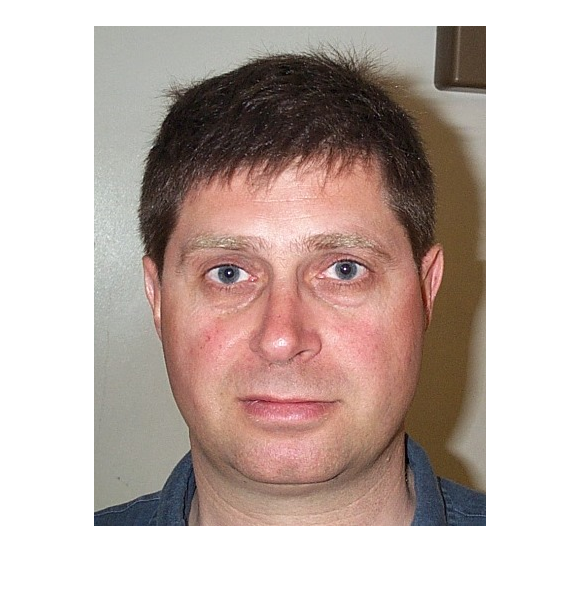
\includegraphics[width=0.8\textwidth]{img/blur_test/orig_img.png}
  \caption{}
\end{subfigure}%
\begin{subfigure}{.30\textwidth}
  \centering
  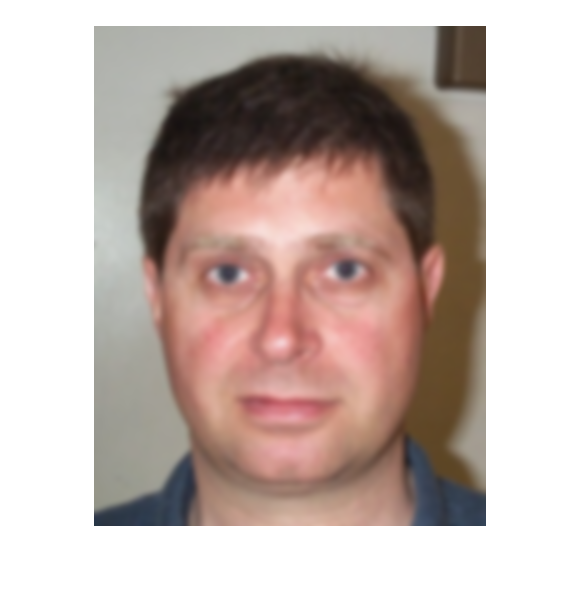
\includegraphics[width=0.8\textwidth]{img/blur_test/gauss_img.png}
  \caption{}
\end{subfigure}%
\begin{subfigure}{.30\textwidth}
  \centering
  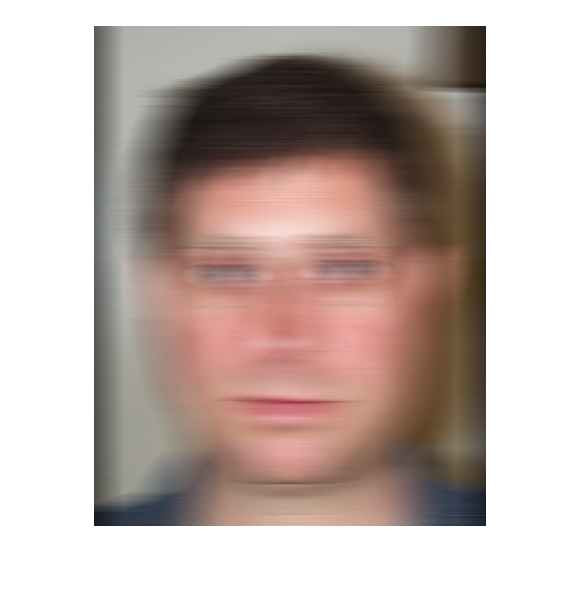
\includegraphics[width=0.8\textwidth]{img/blur_test/motion_img.png}
  \caption{}
\end{subfigure}%
\caption{A comparison of different types of blur applied to the same image. (a) shows the original image. (b) shows the effect of applying Gaussian blur to (a) using a standard deviation of 3.0. (c) shows the result of a 60 pixels wide linear motion blur filter applied to (a).}
\label{fig:fr_result_images}
\end{figure}

To compare LPQ to Eigenfaces another set of tests where performed where the tone value of the input images varied. This was claimed to be an issue for Eigenfaces, but the tests performed showed that LPQ could handle it without reducing performance significantly. Some of the tests even suggested that decreasing the tone value could improve recognition rates by a few percent. This may be caused by some oversaturated images that are matched to the correct descriptor but whose distance value is above to allowed threshold. By reducing the tone value the distance between the descriptors are also effected so that these image now pass as they should.

An area of improvement for the face recognition algorithm is how the threshold that determines whether or not an image should be considered a math is chosen. Currently this value is chosen by conducting a number of tests with images that have no match and choosing a threshold so that no match is found for any of these images. If the Eigenfaces method had been chosen over LPQ a more accurate way of determining this would have been possible. Eigenfaces revolves around finding a subspace for all descriptors of the images in the database and therefore the boundary of this subspace can be used as a threshold. This is unfortunately not possible for LPQ.
